\documentclass[11pt,]{article}
\usepackage[left=1in,top=1in,right=1in,bottom=1in]{geometry}
\newcommand*{\authorfont}{\fontfamily{phv}\selectfont}
  \usepackage[]{mathpazo}
  
  
  \usepackage[T1]{fontenc}
\usepackage[utf8]{inputenc}




\usepackage{abstract}
\renewcommand{\abstractname}{}    % clear the title
\renewcommand{\absnamepos}{empty} % originally center

\renewenvironment{abstract}
{{%
  \setlength{\leftmargin}{0mm}
  \setlength{\rightmargin}{\leftmargin}%
}%
  \relax}
{\endlist}

\makeatletter
\def\@maketitle{%
  \newpage
  %  \null
  %  \vskip 2em%
    %  \begin{center}%
    \let \footnote \thanks
  {\fontsize{18}{20}\selectfont\raggedright  \setlength{\parindent}{0pt} \@title \par}%
}
%\fi
\makeatother


  
  
  \setcounter{secnumdepth}{0}

          
    \usepackage{graphicx,grffile}
\makeatletter
\def\maxwidth{\ifdim\Gin@nat@width>\linewidth\linewidth\else\Gin@nat@width\fi}
\def\maxheight{\ifdim\Gin@nat@height>\textheight\textheight\else\Gin@nat@height\fi}
\makeatother
% Scale images if necessary, so that they will not overflow the page
% margins by default, and it is still possible to overwrite the defaults
% using explicit options in \includegraphics[width, height, ...]{}
\setkeys{Gin}{width=\maxwidth,height=\maxheight,keepaspectratio}
  
  
    \title{Transferrability of reflectance-derived models of suspended solids
between nearby estuarine environments  }
  
  
  
  \author{\Large Sean Hardison\vspace{0.05in} \newline\normalsize\emph{University of Virginia}  }
  
  
  \date{}

\usepackage{titlesec}

\titleformat*{\section}{\normalsize\bfseries}
\titleformat*{\subsection}{\normalsize\itshape}
\titleformat*{\subsubsection}{\normalsize\itshape}
\titleformat*{\paragraph}{\normalsize\itshape}
\titleformat*{\subparagraph}{\normalsize\itshape}


  \usepackage{natbib}
\bibliographystyle{apsr}
\usepackage[strings]{underscore} % protect underscores in most circumstances
  
      
  
  \newtheorem{hypothesis}{Hypothesis}
\usepackage{setspace}


% set default figure placement to htbp
\makeatletter
\def\fps@figure{htbp}
\makeatother

  \usepackage{float} \usepackage{longtable} \usepackage{caption}
    
  % move the hyperref stuff down here, after header-includes, to allow for - \usepackage{hyperref}

\makeatletter
\@ifpackageloaded{hyperref}{}{%
  \ifxetex
  \PassOptionsToPackage{hyphens}{url}\usepackage[setpagesize=false, % page size defined by xetex
                                                 unicode=false, % unicode breaks when used with xetex
                                                 xetex]{hyperref}
  \else
    \PassOptionsToPackage{hyphens}{url}\usepackage[draft,unicode=true]{hyperref}
  \fi
}

\@ifpackageloaded{color}{
  \PassOptionsToPackage{usenames,dvipsnames}{color}
}{%
  \usepackage[usenames,dvipsnames]{color}
}
\makeatother
\hypersetup{breaklinks=true,
bookmarks=true,
pdfauthor={Sean Hardison (University of Virginia)},
pdfkeywords = {},  
pdftitle={Transferrability of reflectance-derived models of suspended solids
between nearby estuarine environments},
colorlinks=true,
citecolor=blue,
urlcolor=blue,
linkcolor=magenta,
pdfborder={0 0 0}}
\urlstyle{same}  % don't use monospace font for urls

% Add an option for endnotes. -----


% add tightlist ----------
\providecommand{\tightlist}{%
\setlength{\itemsep}{0pt}\setlength{\parskip}{0pt}}

% add some other packages ----------

% \usepackage{multicol}
% This should regulate where figures float
% See: https://tex.stackexchange.com/questions/2275/keeping-tables-figures-close-to-where-they-are-mentioned
\usepackage[section]{placeins}


\begin{document}
	
% \pagenumbering{arabic}% resets `page` counter to 1 
%
% \maketitle

{% \usefont{T1}{pnc}{m}{n}
\setlength{\parindent}{0pt}
\thispagestyle{plain}
{\fontsize{18}{20}\selectfont\raggedright 
\maketitle  % title \par  

}

{
   \vskip 13.5pt\relax \normalsize\fontsize{11}{12} 
\textbf{\authorfont Sean Hardison} \hskip 15pt \emph{\small University of Virginia}   

}

}








\begin{abstract}

    \hbox{\vrule height .2pt width 39.14pc}

    \vskip 8.5pt % \small 

\noindent Refelctance-based models of water quality are popular due to their high
spatial and temporal coverage, but fall short when \emph{in situ}
validation data are sparse. However, this shortcoming may be mitigated
if water quality models can be effectively generalized to systems with
fewer \emph{in situ} match-ups. To determine the transferrability of
reflectance-based models of total suspended solids (TSS), we first
developed five models of TSS for Chesapeake Bay using MODIS reflectance
data in the 645 nm band. The best performing models were then applied to
model TSS in a nearby coastal bay system along the Atlantic coast of
Virginia where validation data were sparse. Results show that TSS models
were effective for out of sample prediction in Chesapeake Bay, but had
low transferrability to the coastal bays of Virginia. We suggest that
future efforts be made to time water quality measurements in the coastal
bays with satellite fly-overs in order to generate a database of
reflectance validation data. Transferrability could be improved in the
future if the region used to generate training samples were tailored to
be more representative of the hydrodynamic environment of the coastal
bays.


    \hbox{\vrule height .2pt width 39.14pc}


\end{abstract}


\vskip -8.5pt


 % removetitleabstract

\noindent  

\hypertarget{introduction}{%
\section{Introduction}\label{introduction}}

\hypertarget{methods}{%
\section{Methods}\label{methods}}

\hypertarget{total-suspended-solids-data}{%
\subsection{Total suspended solids
data}\label{total-suspended-solids-data}}

Total suspended solids data were queried from water quality databases
hosted by the Chesapeake Bay Program
(\url{https://www.chesapeakebay.net/what/publications_and_data}) and the
Virginia Coast Reserve Long-term Ecological Research (VCR LTER;
\url{https://www.vcrlter.virginia.edu/cgi-bin/showDataset.cgi?docid=knb-lter-vcr.247})
program. In both cases, water samples of pre-determined volume were
filtered through paper filters, dried, and then weighed to estimate the
dry weight of suspended solids in the sample. Only TSS samples collected
in the upper 2 m of the water column were considered in this analysis.
TSS data were collected from 59 monitoring stations in Chesapeake Bay,
and from three stations in the Virginia Coast Reserve (VCR) (Fig. 1). In
both cases, the queried data were limited to samples occurring on the
same day as a MODIS-Terra fly-over between 2000-02-24 and 2020-07-30.

\begin{figure}
\centering
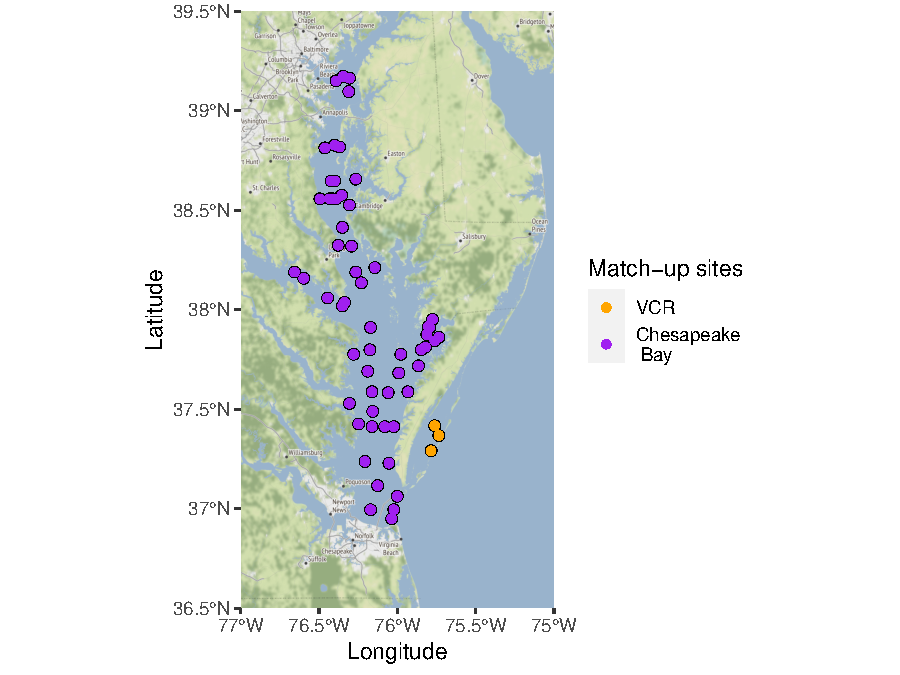
\includegraphics{ssrs_sp2020_files/figure-latex/cb-map1-1.pdf}
\caption{Locations of water quality-MODIS Terra match-up sites in
Chesapeake Bay (orange) and in the Virginia Coast Reserve (purple).}
\end{figure}

\newpage
\singlespacing 
\end{document}